\begin{appendices}

\section*{Abbreviations}

Here we report a list of common abbreviation:

\begin{itemize}
\item \textbf{EOS}: equation of state.
\item \textbf{PV}; parity violating experiment.
\item \textbf{BNSSA}: beam normal single spin asymmetry.
\item \textbf{ENMO}: energy monitor.
\item \textbf{PIMO}: current monitor.
\item \textbf{VFC}: voltage to frequency converter.
\item \textbf{PMT}: photomultiplier tube.
\item \textbf{RTM}: race track microtron.
\item \textbf{XYMO}: position monitor.
\end{itemize} 

\section*{Data Tree}

In this section we discuss briefly the functions implemented to fill the data tree, from the monitor raw values. In the majority of the \transv experiments, the position of the beam respect to the transverse plane is measured in three different position (see next figure). The three monitors are named XY21, XY25, XY26. During this experiment, only two monitors are available, XY25 and XY21, and are used in the analysis. 

\begin{figure}[hbtp]
\centering
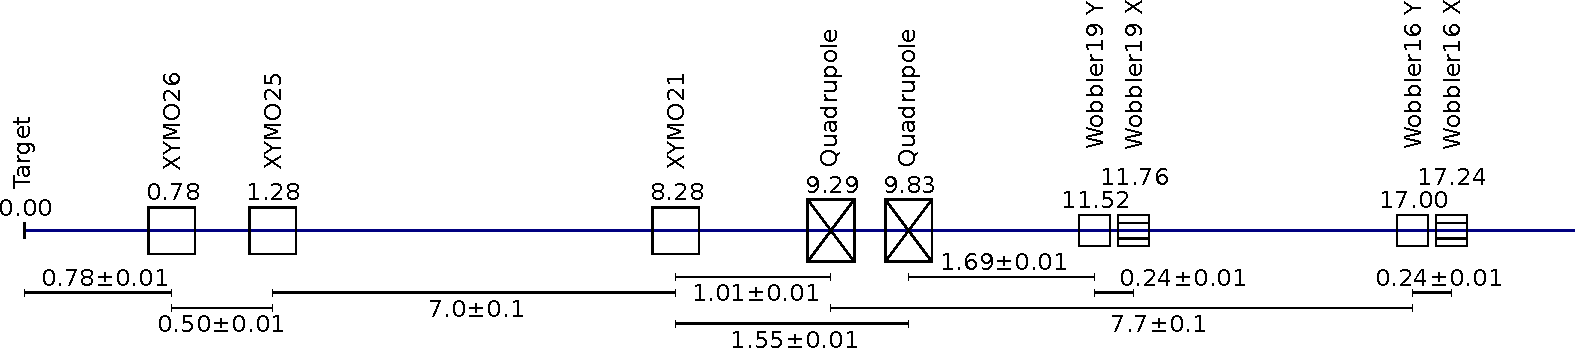
\includegraphics[width = 0.75\textwidth]{figures/XYMOCalibBeamLine.pdf}
\caption{Scheme of the beam line, the target is on the left side of the picture.}
\end{figure}

Other monitors that are used are I21, I13 and E18, the current monitors and energy monitor, respectively. In the figure above, the current monitor I21 correspond to XY21. The E18 monitor, named also ENMO, and I13 are not shown in this picture, because they are placed in the racetrack RTM3 (see figure \ref{fig:Accelerator}). 
The raw values from these monitors and the detectors are collected and stored in binary files produced by the A1 computer. The monitors data and are made by integers numbers, the digital output of the voltage to frequency converter. 
The beam parameters measured by the beam monitors are saved in the class \textit{Beam}, in figure \ref{fig:DataTree}.
The output of the VFCs is proportional to the signal of the beam monitors, as shown in figure \ref{fig:VoltageToFrequency}. The analysis program converts from raw counts to values in \SI{}{\volt} using the formula is given in equation \ref{eq:Vfc}. Once the voltage values are computed, the analysis program does another conversion, from voltage to the physical units. The formula for this conversion is given in \ref{eq:ConversionVoltPhys}:

\begin{equation} \label{eq:ConversionVoltPhys}
\dfrac{V \cdot scale - offset}{I}
\end{equation}

In th formula the coefficient \textit{scale} and \textit{offset} are loaded from the standard configuration files, where all the scaling factors measured during the calibrations are stored.
In the above formula we divide by the beam current $I$, because the output signal of positions and energy the monitors are proportional to the intensity of the beam, and need to be normalized. For the current monitor, the signal is directly proportional to the current, so the denominator is omitted.
The important quantities that are computed by the analysis program are: $X$, $Y$, position of the beam on the target, $\theta_{x}$ and $\theta_{y}$ scattering angles, current $I$ and energy $E$. These quantities are saved in a different class, the \textit{Target} class.
We now briefly present the function implemented to process the raw data and retrieve these quantities.
The position $X$ and $Y$ are computed as explained in section \ref{XYpos}. In brevity, assuming that the beam is moving in a straight line, the  beam trajectory is described by:

\begin{align*}
y &= m_{y} \cdot z + q_{y} \\
x &= m_{x} \cdot z + q_{x}
\end{align*}

The values that we are looking for are $q_{x}$ and $q_{y}$, x and y intercept. 
Imposing in the above equations the passage through the points ($Z_{25}$;$X_{25}$) and ($Z_{21}$;$X_{21}$), the intercepts of the equation are given by:

\begin{equation}
q_{x} = \dfrac{Z_{25} \cdot X_{21} - Z_{21} \cdot X_{25}}{Z_{25} - Z_{21}}
\end{equation} 

The scattering angles $\theta_{x}$ and $\theta_{y}$ are instead related to the slope $m$, knowing that $tan(\theta) = m$. The angles are given by the formula:

\begin{equation}
\theta_{x} = \dfrac{X_{25} - X_{21}}{Z_{25} - Z_{21}}
\end{equation}

With these values, the analysis program compute the differences between different polarization states, that are the independent variables for the linear fit. 
The data tree contains other two classes: detector A and detector B. Each detector class is structured in a number of sub-classes equal to the number of the PMTs, where the counts are stored and processed. The raw data are saved in the variable \textit{rawCounts}, that contains 4 integer number, one for each sub-events. Then the analysis program load the parameters saved in the standard configuration files, where the PMTs offset measured during the auto-calibration are stored. The \textit{offsetCorrectedCounts} are given by equation \ref{eq:OffCorr}

\begin{equation} \label{eq:OffCorr}
offsetCorrectedCounts = rawCounts - N_{i}
\end{equation} 

where $N_{i}$ is the offset measured for PMT i. Other two variables, \textit{positivePolarityCounts} and \textit{negativePolarityCounts} are given by the sum of the offsetcorrectedCounts for sub-events with the same polarization. The \textit{asymmetry} is given by the formula \ref{eq:AsymmFormula}

\begin{equation} \label{eq:AsymmFormula}
asymmetry = \dfrac{(Pc[1] + Pc[2]) - (Nc[1] + Nc[2])}{(Pc[1] + Pc[2]) + (Nc[1] + Nc[2])}
\end{equation}

where $Pc$ and $Nc$ stands for positive and negative polarity counts. 
\end{appendices}